% ============================================================================
% MÓDULO 1 - CAPÍTULO 4: CONCEITOS E DEFINIÇÕES OPERACIONAIS DA ANÁLISE AMBIENTAL
% Componente: CHF662 - Análise Ambiental (DCHF/UEFS)
% Vínculo no Plano CHF662: Semana 4 | Estudo Orientado 3 (EO3) | Prova Teórica
% ============================================================================

\chapter[Conceitos Operacionais da Análise Ambiental]{Conceitos e Definições Operacionais da Análise Ambiental}
\label{cap:conceitos-operacionais}

\noindent\tagEmenta\ \tagEO{3}

\vspace{4pt}

% ============================================================================
% ETAPA 1 - OBJETIVOS DE APRENDIZAGEM
% ============================================================================
\begin{capObjetivos}
Ao concluir este capítulo, você será capaz de:
\begin{enumerate}[leftmargin=1.6em, itemsep=2.5pt]
  \item Definir rigorosamente \textbf{ambiente} e \textbf{meio ambiente} segundo a legislação brasileira (PNMA e CONAMA) e a literatura técnica de referência (Sánchez, 2013; Tauk-Tornisielo, 1996).
  \item Distinguir \textbf{aspecto ambiental} de \textbf{impacto ambiental} na cadeia causa-efeito e classificar impactos segundo natureza, ordem causal, prazo, duração, reversibilidade, abrangência, cumulatividade e sinergia.
  \item Diferenciar com precisão jurídica e técnica \textbf{poluição} e \textbf{degradação ambiental}, reconhecendo casos de degradação sem lançamento de poluentes.
  \item Separar operacionalmente \textbf{perigo ou ameaça ($P$)}, \textbf{vulnerabilidade ($V$)}, \textbf{fragilidade ambiental} e \textbf{risco ambiental ($R = P \times V$)}, executando cálculos matriciais e avaliando variações percentuais de risco após medidas de intervenção.
  \item Comparar \textbf{resiliência}, \textbf{recuperação}, \textbf{restauração}, \textbf{reabilitação} e \textbf{sustentabilidade}, selecionando a estratégia técnica adequada para diferentes passivos ambientais.
\end{enumerate}
\end{capObjetivos}

% ============================================================================
% ETAPA 2 - REVISÃO DE PRÉ-REQUISITOS
% ============================================================================
\begin{capRevisao}
No Capítulo 3, você consolidou a lente epistemológica da Análise Ambiental na Geografia moderna (Geografia Socioambiental de Mendonça e Sistema Tripolar GTP de Bertrand). Agora, o passo seguinte é dominar o \textbf{léxico operacional} usado em laudos técnicos, perícias, licenciamentos e estudos científicos:
\begin{itemize}[leftmargin=1.5em, itemsep=2.5pt]
  \item \textbf{Do conceito amplo à definição operacional,} no debate cotidiano, palavras como ``impacto'', ``poluição'', ``degradação'', ``perigo'' e ``risco'' costumam aparecer como sinônimos imprecisos. Em um Estudo de Impacto Ambiental (EIA) ou em um Plano de Recuperação de Áreas Degradadas (PRAD), confundir esses termos invalida o diagnóstico e compromete decisões legais.
  \item \textbf{Conexão com os próximos módulos,} as definições construídas neste capítulo (com base em Sánchez, 2013, cap. 1, e Tauk-Tornisielo, 1996) fundamentam diretamente a Avaliação de Impacto Ambiental (Cap. 5), a fragilidade de Ross (Cap. 9), o diagnóstico de erosão (Cap. 12), a bioengenharia (Cap. 13) e o PRAD (Cap. 14).
\end{itemize}
\end{capRevisao}

% ============================================================================
% ETAPA 3 - EXPLICAÇÃO TEÓRICA
% ============================================================================
\etapa{3}{Fundamentação Teórica: Vocabulário Operacional, Cadeias Causais e Matriz de Risco}

\begin{boxSimbolo}[Símbolos, Siglas e Convenções do Capítulo]
O arcabouço normativo e técnico deste capítulo articula a \textbf{PNMA} (Política Nacional do Meio Ambiente, Lei nº 6.938/1981), as resoluções do \textbf{CONAMA} (como a Resolução nº 01/1986 sobre impacto ambiental), o \textbf{SNUC} (Lei nº 9.985/2000 sobre recuperação e restauração) e a norma \textbf{ISO 14001} (distinção entre aspecto e impacto). Na avaliação semiquantitativa de riscos, $P$ designa o perigo ou ameaça em escala ordinal de $1$ a $4$ (Baixo a Crítico), $V$ indica a vulnerabilidade socioambiental ou estrutural de $0$ a $4$ (Nula a Muito alta), $R = P \times V$ representa o índice de risco ambiental ($0$ a $16$) e $\Delta R\%$ mede sua variação percentual após medidas preventivas ou mitigadoras.
\end{boxSimbolo}

\section{Ambiente e Meio Ambiente: Enquadramento Legal e Científico}

Na legislação brasileira, a Política Nacional do Meio Ambiente (Lei nº 6.938/1981, Art. 3º, inciso I) define \textbf{meio ambiente} como o ``conjunto de condições, leis, influências e interações de ordem física, química e biológica, que permite, abriga e rege a vida em todas as suas formas''. Essa definição marcou um avanço histórico ao reconhecer o caráter sistêmico e interativo do ambiente, superando a lista estática de elementos isolados.

Na prática da Análise Ambiental contemporânea, conforme destacam Sánchez (2013, cap. 1) e Tauk-Tornisielo (1996), o conceito operacional de \textbf{ambiente} precisa ser lido de forma ampliada, abrangendo tanto o meio natural (físico e biótico) quanto o meio construído e as relações socioeconômicas e culturais. Essa ampliação é confirmada pela própria Resolução CONAMA nº 01/1986, que ao regulamentar a Avaliação de Impacto Ambiental exige o diagnóstico integrado de três meios, compreendendo o \textit{meio físico} (subsolo, água, ar, clima, relevo e solos), o \textit{meio biológico e ecossistemas naturais} (fauna, flora e interações ecológicas) e o \textit{meio socioeconômico} (uso e ocupação do solo, infraestrutura, economia local, patrimônio histórico e cultural).

\section{Aspecto Ambiental, Impacto Ambiental e Classificação de Impactos}

Um dos avanços conceituais mais importantes da gestão ambiental moderna, consolidado pela norma ABNT NBR ISO 14001 e sistematizado por Sánchez (2013), consiste na separação rigorosa entre \textbf{atividade}, \textbf{aspecto ambiental} e \textbf{impacto ambiental} em uma cadeia causal contínua (Figura~\ref{fig:aspecto-risco}, Subfigura (a)). A \textbf{atividade humana} funciona como causa geradora, englobando toda ação, obra, processo produtivo ou serviço executado pela sociedade, como a abertura de estrada em encosta, a operação de um laticínio, a terraplanagem de um parque eólico ou a implantação de uma estação de tratamento de esgoto. Dessa atividade deriva o \textbf{aspecto ambiental}, isto é, o mecanismo de interação pelo qual elementos das atividades, produtos ou serviços entram em contato com o meio ambiente, a exemplo da supressão da cobertura vegetal com exposição do solo à chuva, do lançamento de efluente líquido com carga orgânica, da emissão de poeira ou da captação de água subterrânea. Como consequência desse contato surge o \textbf{impacto ambiental}, definido pela Resolução CONAMA nº 01/1986 (Art. 1º) e por Sánchez (2013) como qualquer alteração das propriedades físicas, químicas e biológicas do meio ambiente resultante das atividades humanas que afete a saúde, a segurança, o bem-estar da população, as atividades sociais e econômicas, a biota, as condições estéticas e sanitárias ou a qualidade dos recursos ambientais.

Diferentemente do senso comum, no qual ``impacto'' costuma aparecer como sinônimo de prejuízo, na Análise Ambiental técnica o impacto corresponde a qualquer alteração da qualidade ambiental produzida por ação humana, podendo assumir caráter \textbf{adverso (negativo)}, quando degrada o meio, ou \textbf{benéfico (positivo)}, quando melhora condições ecológicas ou socioeconômicas, como na recomposição de mata ciliar ou na implantação de saneamento básico. A cadeia causal da atividade ao impacto articula-se diretamente com a matriz conceitual de risco ambiental (Figura~\ref{fig:aspecto-risco}), cuja estrutura $4 \times 4$ será detalhada na seção sobre risco.

\begin{figure}[htbp]
  \centering
  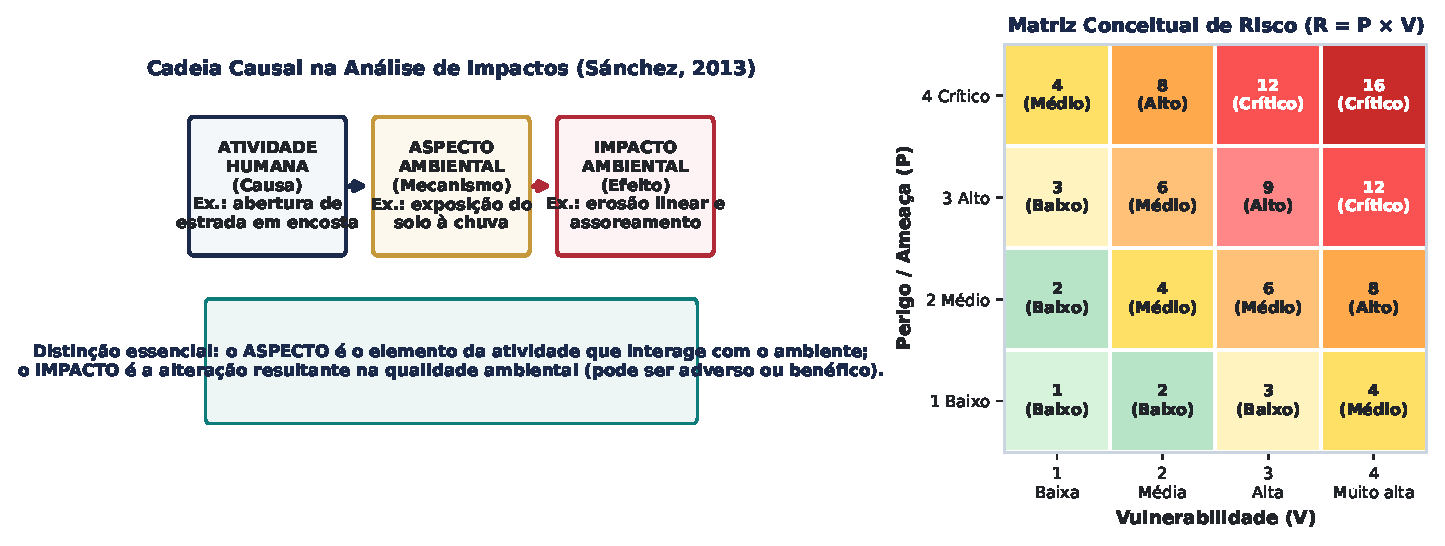
\includegraphics[width=0.95\textwidth]{figures/fig02_aspecto_impacto_risco.pdf}
  \caption{Conceitos operacionais centrais da Análise Ambiental: (a) cadeia causal Atividade Humana, Aspecto Ambiental e Impacto Ambiental segundo Sánchez (2013); (b) Matriz Conceitual de Risco Ambiental ($R = P \times V$) em escala ordinal $4 \times 4$ (Baixo, Médio, Alto e Crítico). Fonte: Elaboração didática CHF662.}
  \label{fig:aspecto-risco}
\end{figure}

Para que os impactos identificados em um diagnóstico sejam comparáveis e subsidiem medidas mitigadoras proporcionais, a Análise Ambiental classifica cada impacto segundo sete atributos operacionais (Sánchez, 2013). Quanto à \textbf{natureza (valor)}, distingue-se o impacto adverso (como erosão em sulcos após desmatamento) do benéfico (como o aumento da infiltração após bioengenharia de talude). Quanto à \textbf{ordem causal}, separa-se o impacto direto ou primário (remoção da vegetação em margem) do indireto ou secundário (assoreamento a jusante reduzindo o volume útil de um reservatório). Pelo \textbf{prazo de manifestação}, diferencia-se o efeito imediato (ruído e poeira durante uma obra) daquele de médio ou longo prazo (salinização progressiva de solo irrigado no Semiárido). Quanto à \textbf{duração}, o impacto pode ser temporário (turbidez restrita à construção de um bueiro), permanente (submersão definitiva de um vale por barragem) ou cíclico. Quanto à \textbf{reversibilidade}, distinguem-se alterações reversíveis mediante manejo (compactação superficial) daquelas irreversíveis (extinção local de espécie endêmica ou perda total de horizonte orgânico em rocha exposta). Pela \textbf{abrangência espacial}, classifica-se o efeito em local ou pontual, regional (alteração hidrológica na bacia do Rio Paraguaçu) ou estratégico. Ademais, quanto à \textbf{interação e acumulação}, o impacto \textbf{cumulativo} resulta da soma de efeitos semelhantes ao longo do tempo ou de múltiplos empreendimentos (como dezenas de pequenos barramentos reduzindo a vazão total de um rio), enquanto o impacto \textbf{sinérgico} decorre da interação entre dois ou mais impactos distintos cujo efeito combinado supera a soma isolada das partes (como supressão de mata ciliar associada ao lançamento de esgoto doméstico elevando drasticamente a eutrofização e o assoreamento). O Exemplo 4.1 aplica essa cadeia causal e sua classificação a uma obra viária urbana.

\begin{boxExemplo}{4.1 (Básico)}{Cadeia Atividade-Aspecto-Impacto e Classificação em Obra Urbana}
\passoEnunciado{A prefeitura de Feira de Santana realiza uma obra de abertura de avenida marginal com drenagem pluvial ao longo de um córrego urbano. Durante a terraplanagem em período chuvoso, máquinas retiram a vegetação de barranco sem instalar barreiras de contenção de sedimentos, gerando enxurrada barrenta que atinge o córrego e assoreia um trecho de $400\text{ m}$ a jusante. Estruture a cadeia causal e classifique o impacto de assoreamento.}
\passoDados{Obra de abertura de avenida marginal; retirada de vegetação e exposição de solo sem contenção durante chuvas; carreamento de sedimentos e assoreamento de $400\text{ m}$ do córrego a jusante.}
\passoPedido{Separar atividade, aspecto ambiental e impacto ambiental (direto e indireto), classificando o assoreamento pelos critérios de Sánchez (2013).}
\passoMetodo{Cadeia causal da Figura~\ref{fig:aspecto-risco} (Sánchez, 2013) e os sete atributos operacionais de classificação de impactos.}
\passoContas{%
\textbf{Passo 1, Cadeia causal.} A \textbf{atividade humana} é a terraplanagem para abertura da avenida marginal. O \textbf{aspecto ambiental} consiste na supressão da cobertura vegetal com exposição do solo solto à ação erosiva da chuva e carreamento de partículas para a drenagem. O \textbf{impacto ambiental direto} corresponde à erosão acelerada no talude da obra e ao aumento imediato da turbidez da água, desencadeando o \textbf{impacto ambiental indireto} de assoreamento da calha do córrego ao longo de $400\text{ m}$ a jusante, com redução da seção de escoamento e maior risco de transbordamento.\\
\textbf{Passo 2, Classificação do impacto ``assoreamento a jusante''.} O efeito apresenta natureza \textbf{adversa}, ordem causal \textbf{indireta} (decorrente da erosão no talude), prazo \textbf{imediato a médio prazo} (já nas primeiras chuvas intensas), duração \textbf{temporária a permanente} (enquanto faltarem desassoreamento e estabilização da margem), caráter \textbf{reversível} mediante manejo corretivo (contenção de taludes e remoção controlada de sedimentos), abrangência \textbf{local} ($400\text{ m}$ na microbacia urbana) e comportamento \textbf{cumulativo} ao somar-se a sedimentos de outros loteamentos na mesma bacia.}
\passoResposta{Atividade definida pela terraplanagem; Aspecto definido pela exposição de solo sem contenção; Impacto direto em erosão e turbidez; Impacto indireto em assoreamento a jusante (adverso, indireto, imediato a médio prazo, reversível mediante intervenção, local e potencialmente cumulativo).}
\passoVerificacao{A separação clara entre aspecto e impacto permite atacar a causa (instalar barreiras de contenção, biomantas e drenagem provisória sobre o solo exposto) antes que o assoreamento se consolide.}
\end{boxExemplo}

Trocar o mecanismo de interação (aspecto) pela alteração ambiental resultante (impacto) é uma das falhas mais comuns em matrizes de Avaliação de Impacto Ambiental, como aponta o Erro 1.

\begin{boxErro}[Erro 1: Confundir Aspecto Ambiental com Impacto Ambiental]
\textbf{Equívoco frequente:} listar em uma matriz de AIA o ``desmatamento'' ou o ``lançamento de esgoto'' na coluna de \textit{impactos ambientais}.

\textbf{Por que está incorreto:} desmatamento (supressão vegetal) e lançamento de esgoto são \textbf{aspectos ambientais} (mecanismos pelos quais a atividade interage com o meio). Os \textbf{impactos} são as alterações resultantes na qualidade ambiental, como perda de habitat, erosão laminar, redução do oxigênio dissolvido ou mortandade de peixes.

\textbf{Como evitar:} teste sempre a frase com o conector ``provoca'', verificando que a \textit{Atividade} gera o \textit{Aspecto}, que \textbf{provoca} o \textit{Impacto}.
\end{boxErro}

\section{Poluição versus Degradação Ambiental}

A Lei nº 6.938/1981 (Art. 3º, incisos II e III) e Sánchez (2013) estabelecem uma relação lógica precisa de gênero e espécie entre degradação ambiental e poluição. A \textbf{degradação da qualidade ambiental} corresponde ao gênero, definido como a \textit{alteração adversa} das características do meio ambiente por meio de processos físicos, químicos ou biológicos que reduzem a qualidade ecológica, a produtividade do solo, a estabilidade do relevo ou a funcionalidade dos ecossistemas. Dentro desse conjunto mais amplo situa-se a \textbf{poluição} como espécie particular, caracterizada pela degradação da qualidade ambiental resultante de atividades que prejudiquem a saúde, a segurança e o bem-estar da população, criem condições adversas às atividades sociais e econômicas, afetem desfavoravelmente a biota ou as condições estéticas e sanitárias do meio ambiente, ou \textit{lancem matérias ou energia em desacordo com os padrões ambientais estabelecidos}.

Na prática pericial, \textbf{toda poluição causa degradação ambiental, enquanto a degradação ambiental também ocorre sem lançamento de poluentes}. Assim, o desmatamento ilegal de uma encosta de Caatinga seguido de sobrepastejo provoca compactação do solo, perda de biodiversidade e erosão em ravinas, configurando severa \textbf{degradação ambiental} mesmo na ausência de substâncias tóxicas ou poluentes químicos. Já o despejo de efluente industrial com metais pesados em um córrego acima dos padrões do CONAMA caracteriza simultaneamente \textbf{poluição} e \textbf{degradação ambiental}. O Exemplo 4.2 aplica essa distinção a duas propriedades rurais vizinhas.

\begin{boxExemplo}{4.2 (Básico)}{Poluição vs. Degradação Ambiental em Duas Propriedades no Semiárido}
\passoEnunciado{Durante fiscalização técnica em uma sub-bacia do Semiárido baiano, um analista avalia duas propriedades rurais vizinhas. Na Propriedade Alfa, o superpastejo contínuo removeu o estrato herbáceo, compactou o solo e desencadeou sulcos e ravinas profundas em encosta. Na Propriedade Beta, um pequeno laticínio lança soro de leite e água de lavagem sem tratamento diretamente em um riacho intermitente, elevando a Demanda Bioquímica de Oxigênio (DBO) muito acima dos limites do CONAMA e provocando mortandade de peixes nas poças remanescentes. Classifique cada situação quanto a degradação ambiental e poluição.}
\passoDados{Propriedade Alfa com superpastejo, solo compactado e erosão em ravinas sem lançamento de substâncias químicas ou efluentes. Propriedade Beta com lançamento de efluente orgânico fora dos padrões legais, elevação de DBO e mortandade de peixes.}
\passoPedido{Determinar, com base na Lei nº 6.938/1981 e em Sánchez (2013), se cada caso caracteriza degradação ambiental, poluição ou ambos.}
\passoMetodo{Aplicação dos incisos II e III do Art. 3º da PNMA (gênero dado pela degradação e espécie dada pela poluição).}
\passoContas{%
\textbf{Passo 1, Análise da Propriedade Alfa.} Ocorre alteração adversa severa das propriedades físicas e ecológicas do solo (compactação, perda de cobertura e erosão em ravinas), sem lançamento de substância poluente em desacordo com padrões de emissão. Caracteriza-se, portanto, \textbf{degradação ambiental} sem poluição em sentido estrito.\\
\textbf{Passo 2, Análise da Propriedade Beta.} Ocorre lançamento de matéria orgânica em desacordo com os padrões ambientais vigentes, afetando desfavoravelmente a biota (mortandade de peixes) e as condições sanitárias da água. Como toda poluição constitui uma forma específica de degradação, o caso reúne simultaneamente \textbf{poluição hídrica} e \textbf{degradação ambiental}.}
\passoResposta{Propriedade Alfa apresenta degradação ambiental sem poluição. Propriedade Beta apresenta poluição hídrica e, consequentemente, degradação ambiental.}
\passoVerificacao{O enquadramento jurídico e técnico está consistente com a relação de inclusão da PNMA ($\text{poluição} \subset \text{degradação}$), orientando respostas distintas, como manejo conservacionista do solo e pastagem em Alfa e estação de tratamento de efluentes com autuação por poluição em Beta.}
\end{boxExemplo}

Igualar poluição e degradação ou negar a existência de impactos positivos gera enquadramentos jurídicos equivocados, como detalhado no Erro 2.

\begin{boxErro}[Erro 2: Tratar Todo Impacto como Negativo e Igualar Poluição a Degradação]
\textbf{Equívoco frequente:} afirmar que ``não há impacto ambiental em projetos de recuperação'' ou dizer que ``a erosão do solo por pastoreio é um caso de poluição''.

\textbf{Por que está incorreto:} projetos de recuperação geram \textbf{impactos ambientais benéficos} (positivos); além disso, erosão sem lançamento de substâncias em desacordo com padrões legais constitui \textbf{degradação ambiental}, distinguindo-se de poluição.

\textbf{Como evitar:} qualifique sempre o impacto (adverso ou benéfico) e verifique se houve lançamento de matéria ou energia ou alteração sanitária prevista no Art. 3º, III da PNMA antes de usar o termo poluição.
\end{boxErro}

\section{Perigo, Vulnerabilidade, Fragilidade Ambiental e Risco Ambiental}

Quatro conceitos frequentemente confundidos em relatórios técnicos precisam ser rigorosamente separados para fundamentar mapas de risco, defesa civil e ordenamento territorial, cuja lógica matricial foi introduzida na Subfigura (b) da Figura~\ref{fig:aspecto-risco}. O \textbf{perigo ou ameaça ($P$)} designa o evento ou fenômeno físico, biológico ou tecnológico com potencial intrínseco de causar dano a pessoas, bens ou ecossistemas (como chuva extrema concentrada, escorregamento translacional em encosta, inundação brusca ou rompimento de barragem), referindo-se à \textit{probabilidade e intensidade do evento potencialmente danoso}.

Diante dessa ameaça, a \textbf{vulnerabilidade ($V$)} mede o grau de exposição, suscetibilidade e incapacidade de proteção, resposta ou recuperação de uma população, edificação, infraestrutura ou atividade econômica. Trata-se de um atributo com forte componente socioespacial, pois famílias com moradias precárias em fundos de vale sem drenagem nem alerta precoce apresentam vulnerabilidade muito superior à de edificações estruturadas fora da cota de inundação diante da mesma chuva. Já a \textbf{fragilidade ambiental} expressa uma propriedade física e ecológica intrínseca de um ambiente ou unidade de paisagem de sofrer desestabilização frente a processos morfodinâmicos e intervenções humanas, em função da interação entre declividade, solo, litologia, clima e cobertura vegetal (conceito formalizado no Cap.~9 com a metodologia de Ross, 1994), subsistindo mesmo quando falta ocupação humana.

Dessa articulação emerge o \textbf{risco ambiental ($R$)}, entendido como a expectativa de perdas ou danos resultante da interseção entre um \textbf{perigo ($P$)} e um sistema \textbf{vulnerável ($V$)}. A distinção entre fragilidade física e risco socioambiental evidencia-se quando comparamos duas encostas com idêntica declividade de $38\%$ e solo raso (Figura~\ref{fig:risco_vs_fragilidade}). Enquanto a Vertente~1 permanece conservada e sem população exposta ($V = 0 \Rightarrow R = 0$), na Vertente~2 o desmatamento e a ocupação irregular na base elevam o perigo e a vulnerabilidade até o risco crítico ($R = 16$).

\begin{figure}[H]
  \centering
  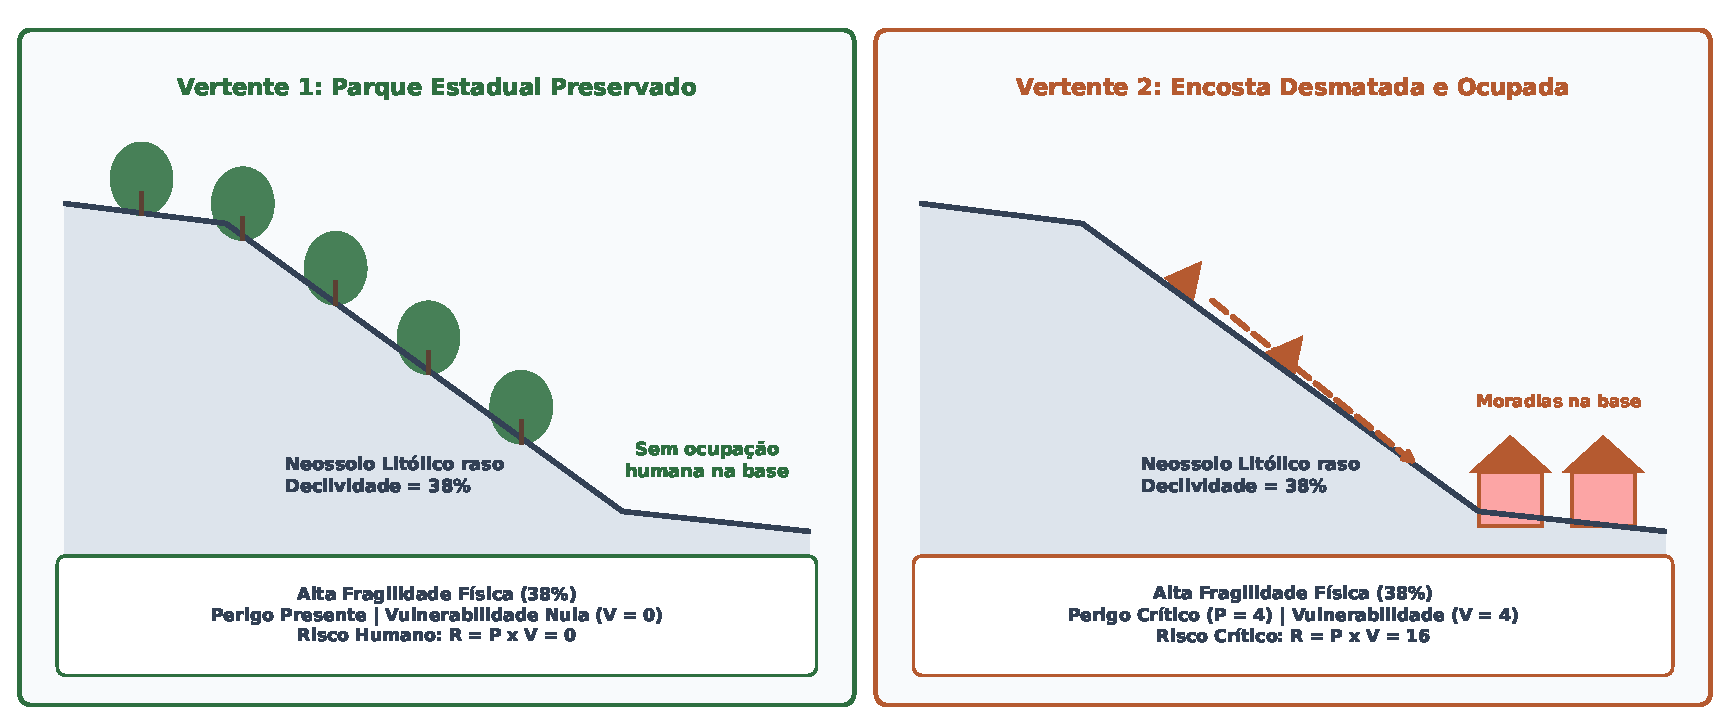
\includegraphics[width=0.95\textwidth]{figures/fig_cap04_risco_vs_fragilidade.pdf}
  \caption{Distinção operacional entre fragilidade física, perigo, vulnerabilidade e risco ($R = P \times V$) em duas encostas com mesma declividade de 38\% e solo raso, contrastando risco humano nulo na Vertente 1 ($V = 0$) e risco crítico na Vertente 2 ($R = 16$). Fonte: Elaboração didática CHF662.}
  \label{fig:risco_vs_fragilidade}
\end{figure}

Na análise semiquantitativa de riscos socioambientais alinhada à matriz $4 \times 4$ da Subfigura (b) da Figura~\ref{fig:aspecto-risco}, o índice de risco ambiental $R$ resulta do produto entre o nível de perigo ($P$) e o nível de vulnerabilidade ($V$), servindo a redução relativa $\Delta R\%$ para medir o efeito de intervenções preventivas ou mitigadoras. Quando as variáveis são ordinais, o produto $R$ opera como convenção de priorização de gestão, orientando decisões conforme as faixas de risco sem representar probabilidade numérica direta de ocorrência.

\begin{boxFormula}[Equação e Variação Percentual do Risco Ambiental ($R = P \times V$)]
\begin{align}
  R &= P \times V \\
  \Delta R\% &= \frac{R_{\text{final}} - R_{\text{inicial}}}{R_{\text{inicial}}} \times 100\%
\end{align}
Nestas expressões, $P \in \{1, 2, 3, 4\}$ representa o nível de Perigo ($1 = \text{Baixo}$, $2 = \text{Médio}$, $3 = \text{Alto}$, $4 = \text{Crítico}$) e $V \in \{0, 1, 2, 3, 4\}$ indica a Vulnerabilidade ($0 = \text{Nula}$ por ausência de exposição, $1 = \text{Baixa}$, $2 = \text{Média}$, $3 = \text{Alta}$, $4 = \text{Muito alta}$). Os valores de $R$ ($0$ a $16$) agrupam-se nas classes \textbf{Baixo} ($1 \le R \le 3$), \textbf{Médio} ($4 \le R \le 6$), \textbf{Alto} ($8 \le R \le 9$) e \textbf{Crítico} ($R \ge 12$).
\end{boxFormula}

O Exemplo 4.3 demonstra o cálculo matricial do risco em três setores de encosta e quantifica a redução percentual alcançada após obras de drenagem, bioengenharia e realocação.

\begin{boxExemplo}{4.3 (Intermediário)}{Cálculo Matricial e Redução Percentual de Risco Ambiental ($R = P \times V$)}
\passoEnunciado{A Defesa Civil de um município do Recôncavo Baiano mapeou três setores de uma vertente sujeita a escorregamentos (Setores A, B e C) utilizando a matriz $4 \times 4$ da Figura~\ref{fig:aspecto-risco}. Posteriormente, no setor mais grave, a prefeitura executou obras de drenagem superficial, estabilização de talude com bioengenharia e realocação das casas mais precárias. Avalie o risco inicial de cada setor e quantifique o efeito percentual da intervenção.}
\passoDados{Cenário inicial com Setor A ($P = 4$, $V = 4$), Setor B ($P = 3$, $V = 3$) e Setor C ($P = 4$, $V = 1$). Cenário pós-intervenção no Setor A com perigo reduzido de $4$ para $3$ (drenagem e estabilização) e vulnerabilidade reduzida de $4$ para $2$ (realocação e reforço estrutural).}
\passoPedido{Calcular $R = P \times V$ e classificar os setores A, B e C antes da obra, determinando também o novo risco de A e a variação percentual $\Delta R\%$.}
\passoMetodo{Aplicação da equação $R = P \times V$, das faixas da Figura~\ref{fig:aspecto-risco} (1--3 Baixo; 4--6 Médio; 8--9 Alto; 12--16 Crítico) e de $\Delta R\% = \frac{R_1 - R_0}{R_0}\times 100\%$.}
\passoContas{%
\textbf{Passo 1, Cálculo inicial dos três setores.} No Setor A, $R_A = 4 \times 4 = 16$ (\textbf{Risco Crítico}); no Setor B, $R_B = 3 \times 3 = 9$ (\textbf{Risco Alto}); no Setor C, $R_C = 4 \times 1 = 4$ (\textbf{Risco Médio}).\\
\textbf{Passo 2, Comparação crítica entre B e C.} Embora o Setor C possua perigo maior ($P = 4$) do que o Setor B ($P = 3$), seu risco ($R_C = 4$) corresponde a menos da metade do risco de B ($R_B = 9$) porque a vulnerabilidade em C é baixa ($V = 1$).\\
\textbf{Passo 3, Cenário pós-intervenção no Setor A ($P_1 = 3$, $V_1 = 2$).}
\[
R_{A,\text{final}} = 3 \times 2 = 6 \quad (\textbf{Risco Médio}).
\]
\textbf{Passo 4, Variação percentual do risco no Setor A.}
\[
\Delta R\% = \frac{6 - 16}{16} \times 100\% = \frac{-10}{16} \times 100\% = -0{,}625 \times 100\% = -62{,}50\%.
\]}
\passoResposta{Inicialmente, Setor A = $16$ (Crítico), Setor B = $9$ (Alto) e Setor C = $4$ (Médio). Após intervenção no Setor A, $R = 6$ (Médio), representando redução de $62{,}50\%$ no índice de risco.}
\passoVerificacao{O resultado faz pleno sentido matemático ($6/16 = 37{,}5\%$ do risco original, logo queda de $62{,}5\%$) e operacional, demonstrando que atuar simultaneamente sobre o perigo (engenharia e bioengenharia) e sobre a vulnerabilidade (ordenamento e habitação) produz queda acentuada de risco.}
\end{boxExemplo}

Rotular mapas puramente físicos de declividade ou erodibilidade como mapas de risco ignora a dimensão de exposição humana, equívoco alertado a seguir.

\begin{boxErro}[Erro 3: Confundir Fragilidade Ambiental ou Perigo com Risco]
\textbf{Equívoco frequente:} chamar um mapa de declividade ou de erodibilidade de ``mapa de risco ambiental'' sem considerar a presença e a vulnerabilidade da população ou da infraestrutura.

\textbf{Por que está incorreto:} declividade e erodibilidade expressam \textbf{fragilidade} ou \textbf{perigo físico ($P$)}. Sem vulnerabilidade ($V > 0$), falta exposição capaz de gerar risco socioambiental ($R = P \times V$).

\textbf{Como evitar:} verifique se os dois fatores ($P$ e $V$) estão explicitamente presentes no diagnóstico antes de empregar a palavra risco.
\end{boxErro}

O Exemplo 4.4 consolida a separação entre fragilidade potencial, perigo, vulnerabilidade e risco em duas vertentes idênticas da Caatinga sob usos distintos do solo.

\begin{boxExemplo}{4.4 (Intermediário)}{Fragilidade Ambiental vs. Perigo vs. Risco em Vertentes da Caatinga}
\passoEnunciado{Considere duas vertentes geomorfologicamente idênticas no Semiárido baiano, ambas com $38\%$ de declividade, Neossolo Litólico raso e chuvas concentradas de alta erosividade. A Vertente 1 localiza-se no interior de um Parque Estadual preservado, sem estradas nem moradores. A Vertente 2 teve sua vegetação suprimida e recebeu um loteamento residencial irregular na base da encosta. Compare fragilidade ambiental, perigo, vulnerabilidade e risco nas duas vertentes.}
\passoDados{Vertente 1 com declividade $38\%$, solo raso, vegetação de Caatinga preservada e ausência de população ou bens expostos. Vertente 2 com mesma declividade e solo, vegetação suprimida e loteamento irregular na base.}
\passoPedido{Diferenciar conceitualmente a condição de cada vertente quanto a fragilidade potencial, perigo, vulnerabilidade e risco socioambiental.}
\passoMetodo{Distinção rigorosa entre fragilidade intrínseca do meio físico, ameaça física, exposição humana e risco conforme a Seção 4.4.}
\passoContas{%
\textbf{Passo 1, Fragilidade potencial (meio físico).} Ambas as vertentes apresentam \textbf{alta fragilidade natural potencial}, pois compartilham declividade elevada ($38\%$), solo raso e chuvas erosivas. Na Vertente 1, a cobertura vegetal conservada protege o solo (menor fragilidade emergente); na Vertente 2, a supressão vegetal eleva a instabilidade.\\
\textbf{Passo 2, Perigo ou Ameaça ($P$).} Em ambas existe potencial físico de escoamento rápido e queda de material, acentuado na Vertente 2 pela retirada da vegetação e pelos cortes de talude do loteamento.\\
\textbf{Passo 3, Vulnerabilidade ($V$).} Na Vertente 1, faltam pessoas, habitações ou infraestruturas expostas ($V = 0$ do ponto de vista socioambiental humano). Na Vertente 2, há moradias precárias diretamente na zona de impacto ($V$ alta ou muito alta).\\
\textbf{Passo 4, Risco Socioambiental ($R$).} Na Vertente 1, apesar da alta fragilidade física, o risco de desastre humano é \textbf{nulo} ($R = P \times 0 = 0$). Na Vertente 2, a convergência entre alto perigo e alta vulnerabilidade gera \textbf{risco alto ou crítico}.}
\passoResposta{Ambas possuem alta fragilidade física potencial, porém apenas a Vertente 2 apresenta risco socioambiental humano elevado, em virtude da exposição de moradores vulneráveis e da desestabilização antrópica da cobertura vegetal.}
\passoVerificacao{Esse contraste comprova por que mapas de fragilidade física exigem o cruzamento com dados de exposição e vulnerabilidade social antes de receberem o rótulo de ``mapas de risco''.}
\end{boxExemplo}

\section{Resiliência, Recuperação, Restauração, Reabilitação e Sustentabilidade}

Quando um ambiente já sofreu degradação, o analista ambiental precisa avaliar sua capacidade de resposta espontânea e definir o objetivo técnico viável de intervenção, articulando os limiares de tolerância da matriz de risco às trajetórias de resiliência do sistema (Figura~\ref{fig:matriz_risco_tolerancia}). Enquanto níveis baixos de risco ($R \le 3$) demandam monitoramento e níveis médios ($4 \le R \le 6$) requerem controle preventivo, situações de risco alto ($8$ a $9$) exigem mitigação prioritária e riscos críticos ($\ge 12$) impõem intervenção imediata, pois o sistema aproxima-se do limiar de ruptura estrutural.

O ponto de partida dessa avaliação é a \textbf{resiliência}, entendida como a capacidade de um ecossistema ou sistema socioambiental absorver perturbações dentro da faixa de resistência elástica, reorganizar-se e retornar ao estado funcional quando cessa a pressão. Quando a perda de horizontes férteis A e B, a compactação severa ou a incisão em ravinas ultrapassam o \textbf{limiar crítico de ruptura} (ponto de não retorno), o sistema ingressa em um novo estado degradado marcado por \textbf{histerese} (Figura~\ref{fig:matriz_risco_tolerancia}), no qual a mera retirada do fator de pressão falha em recompor o ambiente espontaneamente, exigindo PRAD e bioengenharia.

\begin{figure}[H]
  \centering
  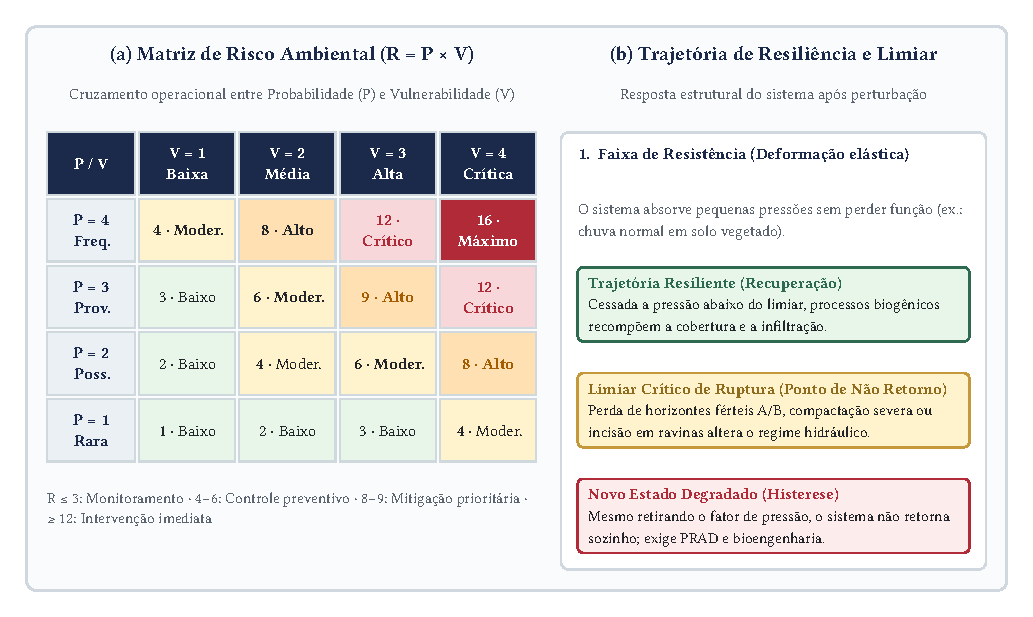
\includegraphics[width=0.95\textwidth]{figures/fig_cap04_matriz_risco_tolerancia.pdf}
  \caption{Articulação entre classes de tolerância e ação na Matriz de Risco Ambiental ($R = P \times V$, Painel (a)) e trajetória de resiliência, limiar crítico de ruptura e histerese após degradação severa (Painel (b)). Fonte: Elaboração didática CHF662.}
  \label{fig:matriz_risco_tolerancia}
\end{figure}

Quando a intervenção humana se torna necessária, Sánchez (2013) e a Lei do SNUC (Lei nº 9.985/2000, Art. 2º, incisos XIII e XIV) diferenciam estratégias com metas técnicas precisas. A \textbf{recuperação ambiental} opera como conceito guarda-chuva técnico e legal adotado em PRAD e licenciamento, designando a restituição de um ecossistema degradado a uma \textit{condição não degradada} que pode igualar-se ou diferir da condição original. Dentro desse espectro, a \textbf{restauração ecológica} representa o objetivo mais exigente, buscando restituir a estrutura, a composição de espécies nativas e as funções ecológicas o mais próximo possível da \textit{condição original pré-distúrbio}, meta indicada para APPs, nascentes e Unidades de Conservação onde a resiliência e os remanescentes permitem recomposição nativa. Já a \textbf{reabilitação ambiental} conduz a área degradada a um estado estável, seguro e funcional voltado a um \textit{novo uso predefinido} (produtivo, urbano, paisagístico ou de lazer) em locais muito alterados, como cavas urbanas ou antigas pedreiras em que o retorno ao estado original é inviável física ou economicamente. Em situações com passivos químicos por hidrocarbonetos, chorume, metais pesados ou agrotóxicos persistentes, aplica-se a \textbf{remediação} (Sánchez, 2013), voltada a remover, conter ou neutralizar contaminantes no solo e na água subterrânea.

Articulando essas escalas no longo prazo, a \textbf{sustentabilidade} atua como princípio orientador que mantém o uso dos recursos naturais dentro da capacidade de suporte e regeneração dos ecossistemas, integrando integridade ecológica, viabilidade econômica, justiça socioespacial e equidade intergeracional. Na literatura ambiental, distingue-se a \textit{sustentabilidade fraca}, que admite substituir capital natural por capital financeiro ou tecnológico, da \textit{sustentabilidade forte}, que reconhece funções ecológicas críticas insubstituíveis, como água doce, solos férteis e biodiversidade.

% ============================================================================
% ETAPA 4 - SÍNTESE AVANÇADA E ESTUDO DE CASO INTEGRADOR
% ============================================================================
\etapa{4}{Síntese Avançada: Resiliência, Sinergia e Escolha de Estratégia em PRAD}

Passivos ambientais severos frequentemente combinam baixa resiliência física, ruptura topográfica irreversível e pressões difusas provenientes do entorno urbano ou agrícola. O Exemplo 4.5 integra os conceitos de resiliência, impacto sinérgico e escolha técnica entre restauração e reabilitação para fundamentar um Plano de Recuperação de Áreas Degradadas.

\begin{boxExemplo}{4.5 (Avançado)}{Escolha entre Restauração e Reabilitação em Passivo Minerário}
\passoEnunciado{Na planície fluvial do Rio Jacuípe (BA), uma área de $8\text{ ha}$ usada por 15 anos para extração irregular de areia deixou cavas com $4\text{ m}$ de profundidade que atingiram o lençol freático, margens instáveis em desmoronamento e perda completa do horizonte A do solo. A área está hoje cercada por expansão urbana e por pequenas lavouras que aplicam fertilizantes solúveis. O Ministério Público exigiu um PRAD. Discuta a resiliência local, o potencial impacto cumulativo e sinérgico com as lavouras vizinhas e justifique tecnicamente a escolha entre restauração ecológica integral e reabilitação ambiental.}
\passoDados{Passivo de $8\text{ ha}$ com cavas de $4\text{ m}$ atingindo o lençol freático, margens instáveis, ausência de solo superficial, entorno urbano e agrícola com fertilizantes e exigência legal de PRAD.}
\passoPedido{Avaliar a resiliência do sistema, a possibilidade de impacto sinérgico com o entorno e a estratégia mais adequada entre restauração e reabilitação.}
\passoMetodo{Critérios de resiliência, impactos cumulativos e sinérgicos e distinção entre recuperação, restauração e reabilitação segundo Sánchez (2013) e Lei do SNUC.}
\passoContas{%
\textbf{Passo 1, Avaliação da resiliência.} A resiliência natural está severamente comprometida (\textbf{muito baixa}). A remoção de $4\text{ m}$ de sedimento eliminou o horizonte superficial, a matéria orgânica e o banco de sementes, alterando irreversivelmente a topografia e expondo a água subterrânea em condição de histerese na qual a regeneração espontânea falha em restituir a floresta ciliar original.\\
\textbf{Passo 2, Impacto sinérgico com as lavouras.} O escoamento superficial carregando nutrientes das lavouras vizinhas (aspecto agrícola) encontra o lençol freático exposto nas cavas estagnadas (aspecto minerário). A combinação desses dois processos distintos gera eutrofização acelerada e risco de contaminação do aquífero, efeito mais intenso do que cada atividade isolada (\textbf{impacto sinérgico}).\\
\textbf{Passo 3, Escolha entre restauração e reabilitação.} A \textbf{restauração ecológica integral} (retorno exato à planície original pré-mineração) exigiria milhões de metros cúbicos de material de aterro externo, criando novas áreas degradadas de empréstimo e tornando-se ambiental e economicamente inviável. A estratégia tecnicamente recomendada é a \textbf{reabilitação ambiental} (inserida no guarda-chuva legal da recuperação), promovendo retaludamento e estabilização das margens das cavas com bioengenharia, implantação de faixa tampão de vegetação nativa ciliar para filtrar nutrientes das lavouras e conversão das lagoas estabilizadas em parque ecológico e área segura de amortecimento hídrico.}
\passoResposta{Resiliência muito baixa; risco de impacto sinérgico (eutrofização e contaminação do aquífero pela interação entre cava aberta e fertilizantes); a estratégia indicada é a \textbf{reabilitação ambiental} associada à faixa tampão vegetada nativa nas bordas, descartando a restauração topográfica integral por inviabilidade física e ecológica.}
\passoVerificacao{A decisão respeita a legislação (o PRAD exige recuperação, que admite reabilitação quando o retorno ao estado original é impraticável) e neutraliza tanto a instabilidade geotécnica das margens quanto a vulnerabilidade do lençol freático.}
\end{boxExemplo}

% ============================================================================
% ETAPA 5 - ARMADILHA CONCEITUAL E MATERIAIS AUDIOVISUAIS DE APOIO
% ============================================================================
\etapa{5}{Armadilha Conceitual e Materiais Audiovisuais de Apoio}

Ao redigir planos de recuperação ou condicionar licenciamentos, um equívoco recorrente consiste em prometer metas tecnicamente inviáveis por confundir o significado jurídico de recuperação, restauração e reabilitação.

\begin{boxErro}[Erro 4: Prometer ``Restauração Integral'' Onde Apenas a Reabilitação é Viável]
\textbf{Equívoco frequente:} redigir em um PRAD que uma cava profunda de mineração ou uma área urbana aterrada será ``integralmente restaurada à sua condição original''.

\textbf{Por que está incorreto:} a restauração exige aproximação máxima da estrutura, composição e funções originais pré-distúrbio, o que frequentemente se torna impossível após alterações geomorfológicas irreversíveis. Promessas inexequíveis levam à rejeição do PRAD ou ao descumprimento de condicionantes.

\textbf{Como evitar:} avalie a resiliência e o grau de alteração do relevo e do solo; adote a \textbf{restauração} apenas quando o retorno ao ecossistema de referência for factível, e a \textbf{reabilitação} quando o objetivo for um novo uso estável e seguro.
\end{boxErro}

Para aprofundar a compreensão integrada dos conceitos de degradação, vulnerabilidade, fragilidade e resiliência ambiental aplicados a estudos técnicos, assista à videoaula recomendada na página da disciplina, intitulada \textit{Degradação Ambiental} (\url{https://www.youtube.com/watch?v=5EFxN7jGob8}), que revisa esses conceitos operacionais e suas implicações para o planejamento e a recuperação de áreas degradadas.

% ============================================================================
% ETAPA 6 - EXERCÍCIOS DE FIXAÇÃO (15 EXERCÍCIOS EM 3 NÍVEIS)
% ============================================================================
\etapa{6}{Exercícios de Fixação}

\subsection*{Nível Básico (Exercícios 1 a 5)}

\begin{enumerate}[leftmargin=1.8em, itemsep=4pt]
  \item Apresente a definição legal de \textbf{meio ambiente} segundo a Lei nº 6.938/1981 (PNMA) e explique por que Sánchez (2013) recomenda incluir explicitamente o meio construído e as relações socioeconômicas na Análise Ambiental.
  \espacoResolucao[2.0cm]

  \item Para a atividade humana ``operação de uma indústria cerâmica de pequeno porte'', cite um exemplo de \textbf{aspecto ambiental} e um exemplo do correspondente \textbf{impacto ambiental}.
  \espacoResolucao[2.0cm]

  \item Explique a diferença entre \textbf{impacto cumulativo} e \textbf{impacto sinérgico}, apresentando um exemplo prático para cada um em uma bacia hidrográfica.
  \espacoResolucao[2.0cm]

  \item Justifique a afirmação segundo a qual toda poluição provoca degradação ambiental, embora a degradação ambiental também ocorra sem poluição.
  \espacoResolucao[2.0cm]

  \item Defina \textbf{resiliência ambiental} e explique por que um solo decapado até a rocha apresenta resiliência muito menor do que uma pastagem abandonada cercada por fragmentos de mata nativa.
  \espacoResolucao[2.0cm]
\end{enumerate}

\subsection*{Nível Intermediário (Exercícios 6 a 10)}

\begin{enumerate}[leftmargin=1.8em, itemsep=4pt, resume]
  \item Uma encosta ocupada (Encosta X) foi avaliada inicialmente com Perigo Alto ($P_0 = 3$) e Vulnerabilidade Muito Alta ($V_0 = 4$). Após obras de retaludamento, drenagem pluvial e melhoria estrutural das moradias, os indicadores caíram para Perigo Médio ($P_1 = 2$) e Vulnerabilidade Média ($V_1 = 2$). Calcule passo a passo o risco inicial $R_0$ e sua classe, o risco final $R_1$ e sua classe, e a variação percentual $\Delta R\%$.
  \espacoResolucao[2.8cm]

  \item Compare duas margens de rio urbano usando a matriz $4 \times 4$ da Figura~\ref{fig:aspecto-risco}, considerando que a \textbf{Margem Y} tem $P = 4$ e $V = 3$, enquanto a \textbf{Margem Z} tem $P = 3$ e $V = 2$. Determine o índice e a classe de risco de cada margem e indique qual delas deve receber prioridade emergencial de intervenção, justificando.
  \espacoResolucao[2.3cm]

  \item A implantação de uma Estação de Tratamento de Esgoto (ETE) municipal gera ruído temporário durante os 8 meses de obras, mas, após entrar em operação, reduz em $85\%$ a carga orgânica lançada no rio local durante décadas. Classifique esses dois impactos segundo os critérios de \textbf{natureza}, \textbf{duração} e \textbf{reversibilidade}.
  \espacoResolucao[2.3cm]

  \item Diferencie \textbf{fragilidade ambiental}, \textbf{perigo} e \textbf{risco} no contexto de um paredão rochoso instável localizado em área desabitada de parque estadual e, em comparação, imediatamente acima de uma rodovia federal movimentada.
  \espacoResolucao[2.3cm]

  \item Uma pedreira de granito desativada na periferia de uma cidade média do Nordeste possui paredões verticais de $18\text{ m}$ e piso totalmente rochoso. Entre \textbf{restauração ecológica} e \textbf{reabilitação ambiental}, qual alternativa é tecnicamente mais adequada? Justifique sua escolha.
  \espacoResolucao[2.3cm]
\end{enumerate}

\subsection*{Nível Aplicado: Questões Objetivas (Exercícios 11 a 15)}

\begin{enumerate}[leftmargin=1.8em, itemsep=5pt, resume]
  \item Na cadeia causal apresentada por Sánchez (2013) e na Figura~\ref{fig:aspecto-risco}, ao analisar a atividade ``aplicação de fertilizantes em área agrícola declivosa'', constitui um \textbf{aspecto ambiental} e o seu respectivo \textbf{impacto ambiental}, nessa ordem:
  \begin{alternativas}
    \item Eutrofização do açude; carreamento de nitrogênio e fósforo pela enxurrada.
    \item Carreamento de nutrientes pela enxurrada para o corpo d'água; eutrofização do açude e proliferação de algas.
    \item Aplicação de fertilizantes; compra de insumos agrícolas.
    \item Proliferação de algas; abertura de estrada rural.
    \item Redução do oxigênio dissolvido; emissão de licença ambiental.
  \end{alternativas}
  \espacoResolucao[1.2cm]

  \item Em uma bacia hidrográfica do Semiárido, cinco pequenas indústrias lançam efluentes tratados dentro do padrão individual, mas a soma das cargas ao longo do rio reduz gradualmente a qualidade da água na foz. Esse fenômeno caracteriza um impacto tipicamente:
  \begin{alternativas}
    \item Benéfico e pontual.
    \item Irreversível e imediato apenas na fonte.
    \item Cumulativo.
    \item Natural e sem origem antrópica.
    \item Estético sem alteração físico-química.
  \end{alternativas}
  \espacoResolucao[1.2cm]

  \item Segundo a Matriz Conceitual de Risco ($R = P \times V$, escala $1$ a $4$ da Figura~\ref{fig:aspecto-risco}), uma área classificada com Perigo Crítico ($P = 4$) e Vulnerabilidade Baixa ($V = 1$) apresenta:
  \begin{alternativas}
    \item $R = 16$ (Risco Crítico).
    \item $R = 12$ (Risco Crítico).
    \item $R = 8$ (Risco Alto).
    \item $R = 4$ (Risco Médio).
    \item $R = 2$ (Risco Baixo).
  \end{alternativas}
  \espacoResolucao[1.2cm]

  \item De acordo com a Lei do SNUC (Lei nº 9.985/2000) e com Sánchez (2013), a restituição de um ecossistema degradado a uma condição \textbf{o mais próximo possível da sua condição original} denomina-se:
  \begin{alternativas}
    \item Remediação.
    \item Reabilitação.
    \item Restauração.
    \item Compensação financeira.
    \item Mitigação preventiva.
  \end{alternativas}
  \espacoResolucao[1.2cm]

  \item Sobre o conceito de \textbf{sustentabilidade forte}, em contraste com a sustentabilidade fraca, é correto afirmar que:
  \begin{alternativas}
    \item Admite substituir integralmente ecossistemas críticos por capital financeiro ou infraestrutura artificial.
    \item Reconhece que determinadas funções ecológicas e estoques naturais críticos (como água doce, solos férteis e biodiversidade) são insubstituíveis e impõem limites biofísicos ao crescimento econômico.
    \item Aplica-se exclusivamente a unidades de conservação sem presença humana no entorno.
    \item Desconsidera a justiça social e a dimensão intergeracional na gestão ambiental.
    \item Equivale à compensação pecuniária automática de qualquer dano irreversível.
  \end{alternativas}
  \espacoResolucao[1.2cm]
\end{enumerate}

% ============================================================================
% ETAPA 7 - QUESTÕES ESTILO ENADE E CONCURSOS AMBIENTAIS
% ============================================================================
\etapa{7}{Questões no Estilo ENADE e Concursos Ambientais}

\begin{boxDica}[Estratégia para o Estudo Orientado 3 (EO3) e para a Avaliação Teórica]
No \textbf{EO3} (Semana 4, baseado em Sánchez, 2013, cap. 1, e Tauk-Tornisielo, 1996) e em concursos para Analista Ambiental (IBAMA, ICMBio e INEMA), há três pegadinhas recorrentes que você agora sabe desarmar:
\begin{enumerate}[leftmargin=1.5em, itemsep=1.5pt]
  \item \textbf{Aspecto $\neq$ Impacto,} identificando sempre se o enunciado descreve o mecanismo de interação (aspecto) ou a mudança no estado do meio (impacto).
  \item \textbf{Degradação $\supset$ Poluição,} verificando se houve lançamento de poluente ou alteração sanitária prevista em lei ou apenas degradação física e ecológica (como erosão e desmatamento).
  \item \textbf{Restauração $\neq$ Reabilitação $\neq$ Recuperação,} lembrando que \textit{recuperação} é o termo geral (condição não degradada, igual ou diferente da original), enquanto \textit{restauração} busca o estado original e \textit{reabilitação} destina a área a um novo uso funcional estável.
\end{enumerate}
\end{boxDica}

\begin{enumerate}[leftmargin=1.8em, itemsep=5pt, start=16]
  \item \textbf{(Questão autoral, estilo Concurso Analista Ambiental / IBAMA)} Com base na Política Nacional do Meio Ambiente (Lei nº 6.938/1981), na Resolução CONAMA nº 01/1986 e na obra de Sánchez (2013), julgue as proposições abaixo:
  \begin{enumerate}[label=\Roman*., leftmargin=2.0em, itemsep=2pt]
    \item Um impacto ambiental é necessariamente negativo, razão pela qual programas de recuperação florestal deixam de produzir impactos ambientais.
    \item A remoção da vegetação ciliar com consequente assoreamento de curso d'água constitui degradação ambiental mesmo na ausência de lançamento de efluentes químicos tóxicos.
    \item A interação entre dois impactos distintos cujo efeito conjunto supera a soma de seus efeitos isolados define o caráter sinérgico do impacto.
    \item A exposição do solo decorrente da abertura de uma estrada é o aspecto ambiental, enquanto a perda de solo por erosão laminar e o aumento da turbidez no córrego são os impactos ambientais.
  \end{enumerate}
  Estão corretas apenas as proposições:
  \begin{alternativas}
    \item I e II.
    \item I e III.
    \item II e IV.
    \item II, III e IV.
    \item I, II, III e IV.
  \end{alternativas}
  \espacoResolucao[1.3cm]

  \item \textbf{(Questão autoral, estilo ENADE / Geografia)} Duas comunidades localizam-se na mesma bacia hidrográfica semiárida, submetidas a eventos de enxurrada súbita de igual intensidade (mesmo perigo físico $P = 3$). A Comunidade 1 possui sistema de drenagem pluvial, construções em alvenaria fora da cota máxima de cheia e plano de alerta comunitário ($V = 1$). A Comunidade 2 ocupa precariamente a planície de inundação, sem drenagem nem alerta ($V = 4$). À luz dos conceitos operacionais de perigo, vulnerabilidade e risco ($R = P \times V$), assinale a alternativa correta:
  \begin{alternativas}
    \item Ambas as comunidades possuem o mesmo risco ambiental, pois estão expostas à mesma intensidade pluviométrica ($P = 3$).
    \item A Comunidade 1 apresenta risco baixo ($R = 3$) e a Comunidade 2 apresenta risco crítico ($R = 12$), demonstrando o peso determinante da vulnerabilidade socioespacial na produção de desastres.
    \item A Comunidade 2 apresenta risco médio ($R = 7$), resultado da soma entre perigo ($3$) e vulnerabilidade ($4$).
    \item A vulnerabilidade é uma propriedade estritamente geológica do terreno, independente da renda, da infraestrutura e da localização das moradias.
    \item Para reduzir o risco da Comunidade 2, a única medida tecnicamente possível consiste em modificar o regime climático regional para eliminar a chuva intensa.
  \end{alternativas}
  \espacoResolucao[1.3cm]

  \item \textbf{(Questão autoral, estilo Concurso Perito Ambiental / INEMA)} Um empreendimento de extração de argila abandonou, há dez anos, uma área de $12\text{ ha}$ sem solo superficial, com cavas alagadas e taludes instáveis em periferia urbana. O laudo pericial constatou resiliência natural muito baixa e propôs estabilizar os taludes, revegetar as margens com espécies nativas e integrar o espelho d'água a um parque urbano de retenção de cheias, deixando claro que a reconstituição do relevo e da floresta originais mostra-se inviável. Conceitualmente, a intervenção proposta corresponde à:
  \begin{alternativas}
    \item Restauração ecológica integral, pois utiliza espécies nativas nas margens.
    \item Remediação química, visto que a área estava abandonada há dez anos.
    \item Reabilitação ambiental, modalidade de recuperação que destina a área degradada a um novo uso estável e funcional distinto da condição original.
    \item Degradação controlada, uma vez que preserva a modificação topográfica prévia.
    \item Sustentabilidade fraca ilegal, pois o SNUC proíbe qualquer intervenção que deixe de reconstituir integralmente o estado original.
  \end{alternativas}
  \espacoResolucao[1.3cm]
\end{enumerate}

% ============================================================================
% ETAPA 8 - GABARITO INTEGRALMENTE COMENTADO (EM PÁGINA SEPARADA)
% ============================================================================
\clearpage
\etapa{8}{Gabarito Integralmente Comentado (Exercícios 1 a 18)}

\begin{boxGabarito}[Resolução: Nível Básico (Exercícios 1 a 5)]
\begin{enumerate}[leftmargin=1.8em, itemsep=4pt]
  \item \textbf{Meio ambiente (PNMA e Sánchez, 2013).} Pela Lei nº 6.938/1981 (Art. 3º, I), meio ambiente é o conjunto de condições, leis, influências e interações de ordem física, química e biológica que permite, abriga e rege a vida em todas as suas formas. Sánchez (2013) destaca a inclusão do meio construído e das relações socioeconômicas porque as atividades humanas transformam continuamente os sistemas naturais e os impactos ambientais atingem diretamente a saúde, a economia, o patrimônio e o bem-estar social (como reconhece a Resolução CONAMA nº 01/1986).
  \item \textbf{Indústria cerâmica (aspecto e impacto).} Um exemplo de \textit{aspecto ambiental} é a emissão de fumaça e material particulado pela queima de lenha nos fornos (ou extração de argila em várzea), provocando o \textit{impacto ambiental} de degradação da qualidade do ar e agravo a doenças respiratórias no entorno (ou desestabilização de margens e perda de vegetação ciliar).
  \item \textbf{Cumulativo e Sinérgico.} O impacto \textit{cumulativo} resulta da soma de impactos semelhantes ao longo do tempo ou de diversas fontes (como múltiplos barramentos rurais em uma bacia reduzindo progressivamente a vazão no exutório). O impacto \textit{sinérgico} resulta da interação entre dois ou mais impactos distintos cujo efeito combinado supera a soma isolada das partes (como remoção de mata ciliar somada ao lançamento de esgoto doméstico, acelerando conjuntamente o assoreamento e a eutrofização severa do rio).
  \item \textbf{Poluição $\subset$ Degradação.} Pela PNMA (Art. 3º, II e III), degradação é o gênero (qualquer alteração adversa do meio), enquanto poluição é uma espécie específica de degradação (ligada a prejuízos à saúde, biota ou bem-estar ou lançamento de matéria e energia fora dos padrões). Logo, toda poluição degrada o ambiente, ao passo que processos como desmatamento, compactação e erosão degradam o ambiente sem envolver poluição química.
  \item \textbf{Resiliência.} Capacidade do sistema absorver perturbações e recuperar estrutura e funções essenciais. O solo decapado até a rocha perdeu horizonte orgânico, estrutura porosa, retenção hídrica e banco de sementes (resiliência muito baixa, próxima ao quadro de histerese); já a pastagem cercada por fragmentos nativos preserva solo e fonte próxima de propágulos (sementes e dispersores), conferindo resiliência muito mais alta.
\end{enumerate}
\end{boxGabarito}

\begin{boxGabarito}[Resolução: Nível Intermediário (Exercícios 6 a 10)]
\begin{enumerate}[leftmargin=1.8em, itemsep=4pt, start=6]
  \item \textbf{Cálculo passo a passo do risco na Encosta X.}
  O risco inicial é $R_0 = P_0 \times V_0 = 3 \times 4 = \mathbf{12}$ (\textbf{Risco Crítico}, pois $R \ge 12$). O risco final reduz-se a $R_1 = P_1 \times V_1 = 2 \times 2 = \mathbf{4}$ (\textbf{Risco Médio}, faixa $4 \le R \le 6$). A variação percentual resulta em
  \[
  \Delta R\% = \frac{R_1 - R_0}{R_0} \times 100\% = \frac{4 - 12}{12} \times 100\% = \frac{-8}{12} \times 100\% = -\frac{2}{3} \times 100\% \approx \mathbf{-66{,}67\%}.
  \]
  A intervenção reduziu o índice de risco em $66{,}67\%$, deslocando a encosta da classe Crítica para a classe Média.
  \item \textbf{Comparação Margem Y e Margem Z.}
  A Margem Y alcança $R_Y = 4 \times 3 = \mathbf{12}$ (\textbf{Risco Crítico}), enquanto a Margem Z registra $R_Z = 3 \times 2 = \mathbf{6}$ (\textbf{Risco Médio}). A \textbf{Margem Y} deve receber intervenção emergencial prioritária, pois possui o dobro do índice de risco de Z e encontra-se na faixa crítica ($R = 12$).
  \item \textbf{Classificação dos impactos da ETE.}
  O ruído durante 8 meses de obras apresenta natureza \textbf{adversa}, duração \textbf{temporária} e caráter \textbf{reversível} (cessando ao término da obra). A redução de $85\%$ da carga orgânica no rio apresenta natureza \textbf{benéfica}, duração \textbf{permanente} (enquanto a ETE operar adequadamente) e caráter \textbf{reversível} caso a estação deixe de receber manutenção.
  \item \textbf{Paredão rochoso instável.}
  No parque desabitado, há alta \textbf{fragilidade} física e existência de \textbf{perigo} de queda de blocos ($P > 0$), porém faltam elementos humanos expostos ($V = 0$), resultando em \textbf{risco humano nulo}. Acima da rodovia movimentada, mantêm-se a mesma fragilidade e perigo físico, agora combinados com alta exposição de veículos e passageiros ($V > 0$), configurando \textbf{risco socioambiental elevado} que exige obras de contenção e monitoramento.
  \item \textbf{Pedreira de granito desativada.} A estratégia tecnicamente adequada é a \textbf{reabilitação ambiental}. A remoção de $18\text{ m}$ de maciço rochoso alterou irreversivelmente a topografia e eliminou o solo original, tornando inviável a restauração ecológica à condição pré-mineração. A reabilitação permite estabilizar os paredões, drenar a cava e criar um uso seguro (como parque geológico, anfiteatro ou área de lazer com vegetação rupestre adaptada).
\end{enumerate}
\end{boxGabarito}

\begin{boxGabarito}[Resolução: Nível Aplicado e Estilo ENADE/Concursos (Exercícios 11 a 18)]
\begin{enumerate}[leftmargin=1.8em, itemsep=3.5pt, start=11]
  \item \textbf{Gabarito: (B).} O carreamento de nutrientes pela enxurrada é o mecanismo de interação com o meio (\textit{aspecto}), enquanto a eutrofização e a proliferação de algas representam a alteração na qualidade da água (\textit{impacto}). A alternativa (A) inverte causa e efeito.
  \item \textbf{Gabarito: (C).} A soma de múltiplas contribuições semelhantes ao longo do rio que deteriora gradualmente a qualidade hídrica na foz define o \textbf{impacto cumulativo}.
  \item \textbf{Gabarito: (D).} Pela fórmula $R = P \times V$, temos $R = 4 \times 1 = 4$. Na matriz $4 \times 4$ da Figura~\ref{fig:aspecto-risco}, valores entre $4$ e $6$ correspondem à classe \textbf{Risco Médio}.
  \item \textbf{Gabarito: (C).} A Lei do SNUC (Art. 2º, XIV) define \textbf{restauração} exatamente como a restituição de um ecossistema ou população silvestre degradada o mais próximo possível de sua condição original.
  \item \textbf{Gabarito: (B).} A \textbf{sustentabilidade forte} recusa a substituibilidade plena entre capital natural e capital financeiro, afirmando que funções ecológicas críticas (água, solo e biodiversidade) impõem limites biofísicos reais.
  \item \textbf{Gabarito: (D).} A proposição I é falsa porque impactos ambientais podem ser benéficos (como em programas de recuperação florestal). As proposições II (degradação sem poluente químico), III (definição exata de sinergia) e IV (distinção correta entre aspecto e impacto) estão integralmente corretas.
  \item \textbf{Gabarito: (B).} Comunidade 1 obtém $R_1 = 3 \times 1 = 3$ (Risco Baixo), e Comunidade 2 atinge $R_2 = 3 \times 4 = 12$ (Risco Crítico). Mesmo sob igual perigo ($P = 3$), a vulnerabilidade socioespacial quadruplicou o índice de risco. As demais alternativas usam soma como operação matricial, reduzem vulnerabilidade à geologia ou ignoram medidas de proteção social.
  \item \textbf{Gabarito: (C).} Como a área será estabilizada e destinada a um novo uso funcional (parque de retenção de cheias) sem reconstituição da condição original, trata-se de \textbf{reabilitação ambiental}, uma modalidade legítima de recuperação prevista no escopo de um PRAD.
\end{enumerate}
\end{boxGabarito}

% ============================================================================
% ETAPA 9 - RESUMO DO CAPÍTULO
% ============================================================================
\begin{boxResumo}
\begin{itemize}[leftmargin=1.5em, itemsep=2.2pt]
  \item \textbf{Ambiente,} sistema de interações físico-químicas, bióticas e socioeconômicas (Lei nº 6.938/1981; CONAMA nº 01/1986; Sánchez, 2013).
  \item \textbf{Cadeia Causal,} a Atividade Humana (causa) gera o Aspecto Ambiental (mecanismo), que provoca o Impacto Ambiental (efeito adverso ou benéfico).
  \item \textbf{Atributos dos Impactos,} natureza (adverso ou benéfico), ordem (direto ou indireto), prazo (imediato, médio ou longo), duração (temporário ou permanente), reversibilidade, abrangência espacial, cumulatividade e sinergia.
  \item \textbf{Poluição e Degradação,} degradação é o gênero (toda alteração adversa); poluição é espécie (degradação associada a danos sanitários ou bióticos ou lançamento de matéria e energia fora dos padrões).
  \item \textbf{Fragilidade, Perigo, Vulnerabilidade e Risco,} fragilidade é intrínseca ao sistema biofísico; risco exige interseção entre perigo ($P$) e vulnerabilidade ($V$), calculado na matriz $4 \times 4$ por $R = P \times V$ ($1$--$3$ Baixo; $4$--$6$ Médio; $8$--$9$ Alto; $12$--$16$ Crítico).
  \item \textbf{Resiliência e Intervenção,} \textit{recuperação} (condição não degradada, termo geral) engloba \textit{restauração} (próximo ao original) e \textit{reabilitação} (novo uso funcional estável); \textit{remediação} trata contaminantes químicos; \textit{sustentabilidade forte} respeita limites ecológicos insubstituíveis e evita cruzar o limiar de histerese.
\end{itemize}
\end{boxResumo}

% ============================================================================
% ETAPA 10 - TESTE DE APRENDIZAGEM (CHECKPOINT)
% ============================================================================
\begin{boxTeste}
Responda sem consultar o texto e verifique o gabarito logo abaixo.
\begin{enumerate}[leftmargin=1.6em, itemsep=3pt]
  \item (\textbf{V ou F}) Na Resolução CONAMA nº 01/1986 e em Sánchez (2013), o conceito de impacto ambiental aplica-se exclusivamente a alterações negativas provocadas por atividades industriais.
  \item (\textbf{V ou F}) A compactação do solo e a erosão em sulcos causadas por manejo inadequado de pastagem constituem degradação ambiental, mesmo na ausência de lançamento de poluentes químicos.
  \item \textbf{Cálculo rápido,} na matriz $R = P \times V$ ($1$ a $4$), uma área com $P = 3$ e $V = 3$ recebe qual valor e qual classe de risco? Se a vulnerabilidade for reduzida para $V = 2$ (mantendo $P = 3$), qual será o novo risco e sua classe?
  \item \textbf{Enquadramento técnico,} qual é a diferença central de objetivo entre \textbf{restauração} e \textbf{reabilitação} ambiental?
\end{enumerate}
\vspace{3pt}
\hrule
\vspace{4pt}
{\footnotesize\textbf{Gabarito do Checkpoint:}
\textbf{1.} \F\ (impacto pode ser adverso ou benéfico e resultar de qualquer atividade humana, abrangendo também obras e serviços). \quad
\textbf{2.} \V\ (degradação é o gênero amplo; poluição é espécie particular). \quad
\textbf{3.} Inicial $R = 3 \times 3 = \mathbf{9}$ (\textbf{Risco Alto}); final $R = 3 \times 2 = \mathbf{6}$ (\textbf{Risco Médio}). \quad
\textbf{4.} A \textbf{restauração} busca restituir o ecossistema o mais próximo possível de sua condição original pré-distúrbio; a \textbf{reabilitação} destina a área degradada a um novo uso estável e funcional diferente do original.}
\end{boxTeste}
